\documentclass{article}
\usepackage[utf8]{inputenc}
\usepackage{graphicx}
\usepackage{anysize}
\usepackage{mathtools}
\usepackage{csquotes}
\usepackage{listings}
\usepackage{url}

\lstset{ %
	  numbers=left,                    % where to put the line-numbers; possible values are (none, left, right)
	numbersep=5pt,                   % how far the line-numbers are from the code
}

\usepackage{setspace}
\singlespacing
\onehalfspacing
\doublespacing
\setstretch{1.3} % for custom spacing
\marginsize{2.5cm}{2.5cm}{1cm}{3cm}

\author{
  M.A. de Vos $\quad$
  Q. Stokkink\\
  \small Distributed System group, EEMCS, TUDelft
}
\title{Implementing and deploying experiments using Dispersy and Gumby}

\begin{document}

\maketitle

This document describes how to implement and deploy a distributed experiment using Dispersy and Gumby.
After finishing the assignments in this document, you will be able to to:
\begin{itemize}
	\item Send messages to other users in a peer-to-peer network using Dispersy.
	\item Implement and modify a distributed experiment using Gumby. This includes writing your own scenarios and defining experiment modules.
	\item Deploy and execute your experiment on our DAS-5 supercomputer using Gumby.
\end{itemize}

This tutorial assumes that the reader has a basic understanding of the Python programming language and basic familiarity with git.

\section{Introduction}
Experimentation lies at the heart of science. Experiments are important for verification of hypotheses or to analyse behaviour of algorithms.
Particularly in the field of distributed systems, experiments are often executed at a large scale, involving hundreds of clients producing data and communicating with each other.
Being able to define and run your own experiments is an essential skill.

At the distributed systems department and in particular the blockchain lab~\cite{blockchainlab}, we have created various tools to ease the design and implementation of experiments. In this workshop, we will explore two of these tools, Dispersy and Gumby, and show the practical value of these tools using a basic distributed algorithm that involves cryptographic secret sharing and network communication.
Before turning our attention to the experiment, we will first introduce Dispersy, Gumby and the DAS-5 supercomputer.

\subsection{Dispersy}
Dispersy can be described as a scalable, distributed database, however, it also provides primitives for sending generic messages between users.
Dispersy has the notion of \emph{communities} which are best described as a group of users that share a common goal or objective.
Some examples of available communities are:
\begin{itemize}
	\item SearchCommunity: This community is responsible for keyword search of content within Tribler, our peer-to-peer filesharing software.
	\item MarketCommunity: This community enables peer-to-peer trading and transaction processing.
	\item TrustChainCommunity: This community is the implementation of our scalable blockchain fabric.
\end{itemize}

Creating your own Dispersy community is straightforward and will be demonstrated in this tutorial.
Dispersy is open-source software and can be downloaded from Github\footnote{https://github.com/tribler/dispersy}.
More information about Dispersy can be found in the technical report~\cite{zeilemaker2013dispersy}.

\subsection{Gumby}
Gumby is a framework specifically designed to run experiments.
These experiments can either be executed locally, remotely on a server or on the DAS-5 supercomputer.
Gumby can be downloaded from Github\footnote{https://github.com/tribler/gumby}, however, local experiment execution is only possible on Linux-based environments due to the requirement of the \emph{procfs} file system.
This tutorial will explain the basic concepts in Gumby.

\subsection{DAS-5 Supercomputer}
As you might know, the DAS-5 supercomputer is not a single machine but shared amongst various universities in the Netherlands.
Each university involved in the DAS-5 project hosts a cluster with a fixed amount of nodes.
Detailed information, including the number of nodes on each cluster and hardware specifications, can be found on the DAS-5 website\footnote{http://www.cs.vu.nl/das5/clusters.shtml}.

Since there are many researchers working on large-scale experiments, the DAS-5 has a reservation system where you can reserve some nodes in advance.
This is in particular helpful to make sure that only you are running an experiment on a specific node.
However, the reservation system can be frustrating at times and it might be hard to claim a reservation on time.
Keep this in mind when you might have to run experiments multiple times before conferences or journal deadlines.
Gumby takes care of automatically reserving and releasing nodes during experiments.

\section{Create Your Experiment}
\label{sec:create_experiment}
Now that we introduced Dispersy and Gumby, it is time to see what an experiment looks like and where it is being executed.

\subsection{Jenkins}
Start by opening a web browser and navigate to our Jenkins server, located at  https://jenkins.tribler.org.
Jenkins is open-source software to automate running jobs like tests or experiments.
It is often used during the software development cycle to make sure that software is still stable.
Jenkins jobs can be executed on machines, which are displayed under \emph{Build Executor Status}.
Here you will see an overview of all the machines that are capable of executing Jenkins jobs (these machines are also called \emph{slaves}).
Take a look at the different machines: the slaves that are prefixed with \emph{DAS5\_} are clusters of the DAS-5 supercomputer.
Additionally, some machines running Windows or macOS are available.

Navigate to the \emph{pers} directory on the Jenkins website and locate the job named \emph{workshop\_benaloh\_test}.
We will copy this job so we can modify it accordingly.
To create a copy of an existing job, you should have a valid Jenkins account; if you don't have one, please ask one of the workshop instructors for one.

Start by clicking on the \emph{New Item} in the menu in the upper-left corner of the Jenkins website.
You are now prompted to enter the name of the new job.
Name it something like \emph{workshop\_benaloh\_test\_username} where \emph{username} should be replaced by your Jenkins username or your real name.
Since we copy an existing job, enter the name of this job under the \emph{Copy from} input, at the bottom of the page (which should be \emph{workshop\_benaloh\_test}) and press the \emph{OK} button to create the job.

You will be redirected to the configuration options of the newly created Jenkins job.
Here you can change various settings that are related to your experiment.
Some of the most important experiments will be elaborated now:

\begin{itemize}
	\item \emph{Restrict where this project can be run}: here you specify on which Jenkins slave you wish to run your job. It should be filled with \emph{DAS5\_TUD}, which is the TU Delft cluster of the DAS-5 supercomputer. You can also select other DAS5 clusters here but the default option should work fine.
	\begin{figure}[h!]
		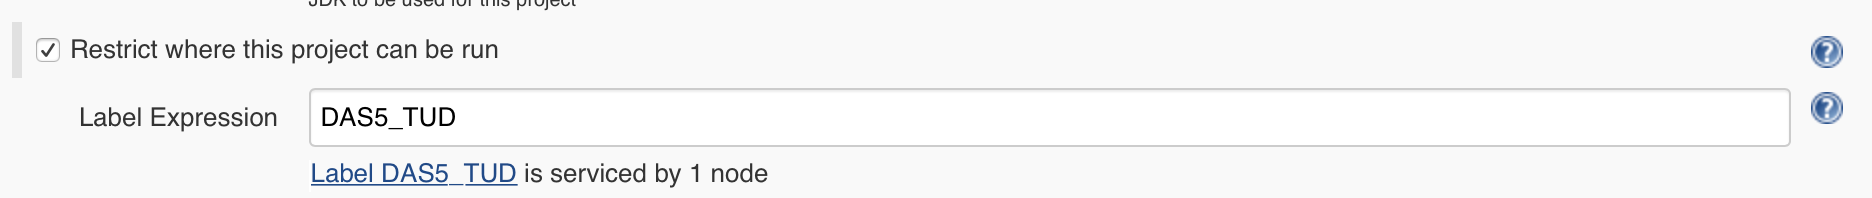
\includegraphics[width=\columnwidth]{jenkins_restrict.png}
	\end{figure}
	\item \emph{Source Code Management}: this section specifies whether the experiment needs some code from external sources like a Version Control System (Git, SVN etc) to operate. Our first option specifies that we are using the workspace of another Jenkins job here (\emph{Clone\_tribler\_devel}). This makes sure that Tribler is downloaded into the Jenkins workspace since Tribler is a dependency of Gumby. Next, we specify that we want to clone a Git repository, namely the Gumby tutorial. The repository URL is specified, including the git branch that we want to checkout. These options together make sure that we have a copy of Tribler and Gumby ready before the experiment starts.
	\begin{figure}[h!]
		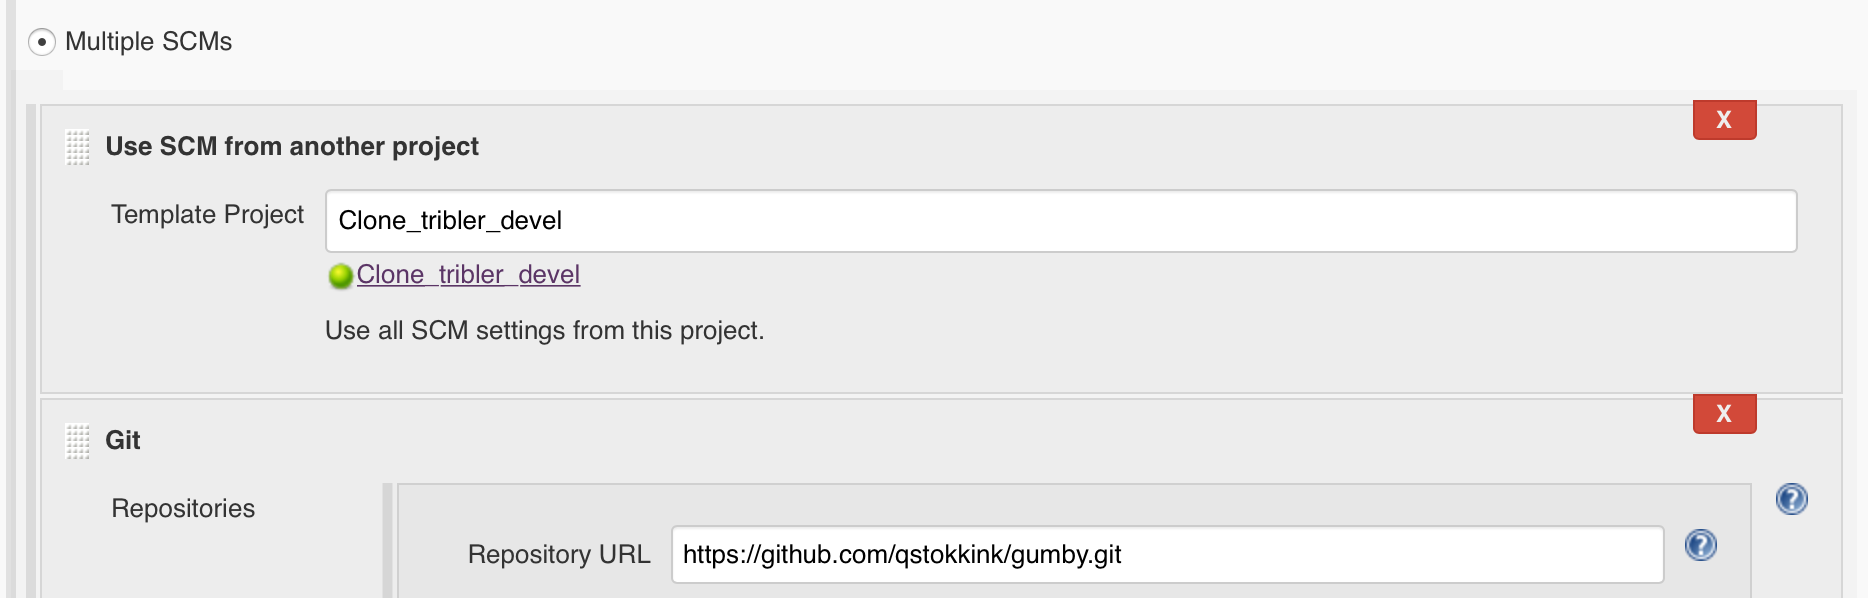
\includegraphics[width=\columnwidth]{jenkins_source.png}
	\end{figure}
	\item \emph{Build}: this section indicates the performed actions during the experiment execution. In this case, we run a simple shell script where activate a virtual Python environment (this makes sure that all required Python libraries can be found but it's not very interesting for now). The final line of the bash script starts the Gumby experiment.
	\begin{figure}[h!]
		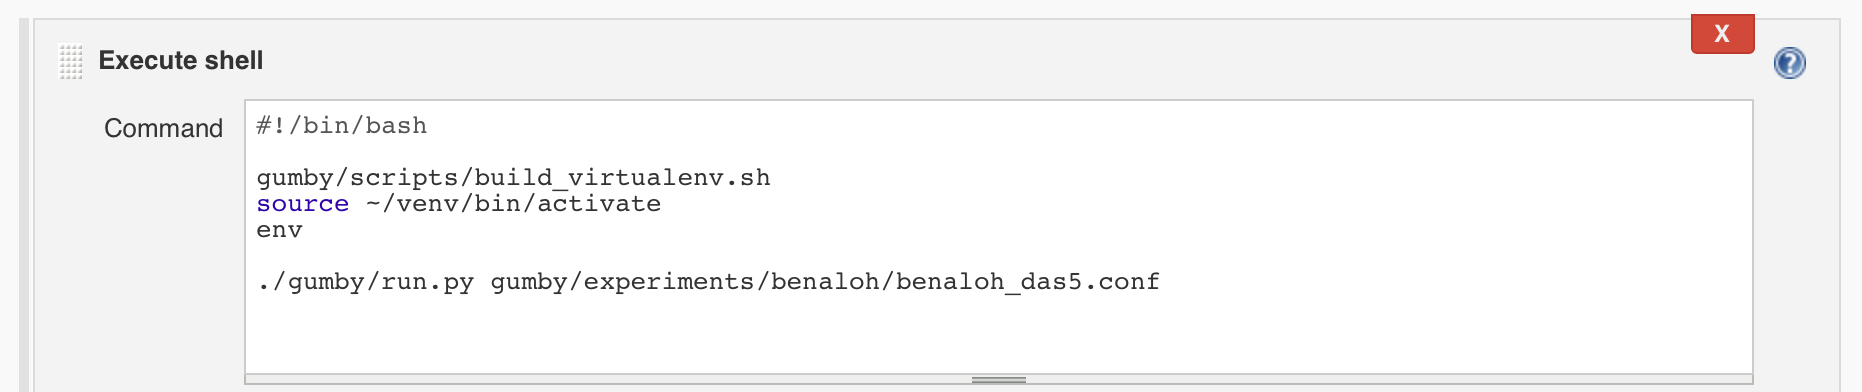
\includegraphics[width=\columnwidth]{jenkins_build.png}
	\end{figure}
	\item \emph{Post-build Actions}: here we specify actions that should be performed after the experiment has finished. In this experiment, we store files in the \emph{output} directory for later usage (this is called archiving). Finally, we create an image gallery from \emph{.png} files.
	\begin{figure}[h!]
		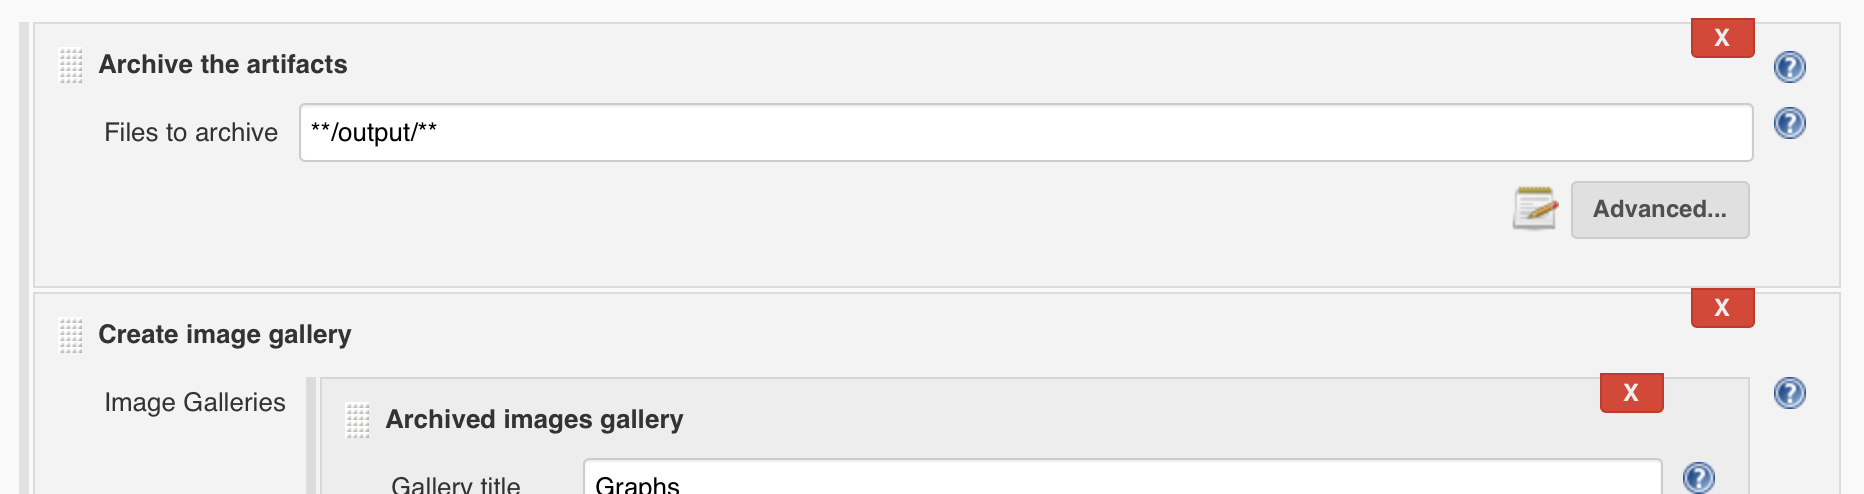
\includegraphics[width=\columnwidth]{jenkins_post_build.png}
	\end{figure}
\end{itemize}

By pressing the \emph{Save} button at the bottom of the webpage, you save the configuration and return to the overview of the specific job.
You can always return to the configuration overview by clicking the \emph{Configure} menu entry.

When executing a job, a new \emph{build} is created.
Each build has a number of outcomes, including \emph{succeeded} (everything went well), \emph{failed} (something went wrong during the execution of the build) or \emph{aborted} (the job got manually or automatically aborted).
The history of builds is presented under the \emph{Build History} tab on the left.
Here you will see the time, outcome and amount of produced data for each build.

\subsection{Running The Experiment}
We are now ready to run your newly created job!
Executing jobs can be done by pressing the \emph{Build Now} button in the upper-left menu, please do so now.
Refresh the web page shortly after pressing the button and you will notice that a new entry appears under the \emph{Build History} overview on the left.
You will see a progress bar that indicates the progress of the build.
Click on the build number to navigate to the page with specific details of each build.
We can monitor the progress of each build in detail by clicking on the \emph{Console Output} menu entry on the left.
The experiment should take several minutes to finish and when it does, you will see something similar to the following lines in the console log:

\begin{lstlisting}[frame=single]  % Start your code-block
Archiving artifacts
Creating image galleries.Creating archived images gallery.No files found for
image gallery.Started calculate disk usage of build
Finished Calculation of disk usage of build in 0 seconds
Started calculate disk usage of workspace
Finished Calculation of disk usage of workspace in 0 seconds
Notifying upstream projects of job completion
Finished: SUCCESS
\end{lstlisting}

This indicates that the build has succeeded.
We can now investigate the output files of the selected build by going to the \emph{Build Artifacts}.
This opens a basic file explorer where you can navigate through all artifacts generated by the build.
The experiment uses five nodes on the DAS-5 supercomputer and each node writes its output to a directory in \emph{output/localhost}\footnote{In actuality the head node of the cluster collects the results of each of the nodes and writes them there.}.
If you navigate to \emph{output/localhost}, you will see five directories.
Click on any of them, for instance, \emph{node301}, to view files produced by this node.
Browse the content of the file named \emph{00000.out} which contains the standard out (stdout) output of the processes running on this DAS-5 node.
You should see the following lines:

\begin{lstlisting}[frame=single]
My computed sum is 656
My secret value is 722
\end{lstlisting}

The computed sum should be the same for all nodes but the secret values are (probably) different.

\section{The Benaloh Experiment}
The output produced in the last section comes from an implementation of a simplified version of the Benaloh secret sharing scheme~\cite{benaloh1990generalized}.
You can find the complete code of this exercise on GitHub\footnote{https://github.com/qstokkink/gumby/tree/workshop\_code/experiments/benaloh}.
In particular we will focus on the different ways to share data and not so much on the security or efficiency of the algorithm.
The protocol is implemented as follows:

\begin{enumerate}
\item Every node starts with a globally known node count $n$ and modulus $M$ and a private share $s$.
The nodes then generate $n-2$ random numbers $R$ and calculates $s - \Sigma R$ individually.
\item Every node shares all values from step $1$ \textbf{directly} with all other nodes.
\item Every node sums all the received values from step $2$ and \textbf{broadcasts} this value to all other nodes.
\item All nodes print the sum of all received values from step $3$.
\end{enumerate}

\noindent We will now explain all components that together form this experiment.

\subsection{The Dispersy Community}
\label{sec:dispersy_community}
Recall that a Dispersy community is a group of users that share a common goal or objective. In this experiment, our objective is secret sharing. The community provides the message definitions to do so.
The source code of this community is given here:

https://github.com/qstokkink/gumby/blob/workshop\_code/experiments/benaloh/benaloh\_community.py

\vspace{\baselineskip}
\noindent Globally this community needs the following components to function:

\begin{itemize}
\item A \texttt{Payload} object, representing packets going over the network.
\item A \texttt{Conversion} object, which can transform \texttt{Payload} objects into binary data.
\item An object that is a subclass of \texttt{Community}, handling incoming \texttt{Payload} objects and providing functionality to send \texttt{Payload} objects to other users in the community.
\end{itemize}

\noindent The finer details of creating these objects will remain out of the scope of this document, but we refer the interested reader to our extensive Dispersy tutorial\footnote{https://dispersy.readthedocs.org}.
For some general clarification, we would now like to draw the attention of the reader to the different types of messages defined in the \\\texttt{BenalohCommunity.initiate\_meta\_messages()} method.

The first type of message you will find defined in the community file is a \textbf{broadcast} message using Dispersy's gossiping: \texttt{u"broadcast-share"}.
This message uses \texttt{MemberAuthentication}, which means that every message will be signed  and verified when received.
The alternative to \texttt{MemberAuthentication} is \texttt{NoAuthentication}.
Next, you will see \texttt{FullSyncDistribution(u"ASC", 128, False)}, this takes care of stamping your message with a global time (a Lamport clock timestamp to be precise \cite{lamport1978time}), which avoids duplicate messages.
Besides this, the \texttt{FullSyncDistribution} definition also serves as a flag to tell Dispersy that your message needs to be gossiped throughout the network.
The \texttt{CommunityDestination(10)} directive then tells Dispersy that your message will be gossiped using a fanout of $10$ neighboring nodes.
Lastly, \texttt{self.on\_broadcast\_share} tells Dispersy which function handles incoming messages of the \\\texttt{u"broadcast-share"} persuasion.

The other message in this file is the \texttt{u"local-share"} message.
This message can be sent directly to other known peers.
You will notice that the difference between the two messages lies in the declaration of the \texttt{DirectDistribution} and \texttt{CandidateDestination}.
These two flags let Dispersy know that you want to directly send this message to others and you will be the one in charge of supplying the peers/candidates to send it to.

One observation you will make is that it is much faster to send to other candidates directly instead of gossiping it (using the broadcast message).
Still, it would not be wise, even erroneous, to use the direct candidate sending, as given by the supplied code, outside of Gumby.

\subsection{The Gumby Experiment}
Now that you know how a basic Dispersy community works and that you understand messaging between nodes, we should focus on the Gumby experiment that uses the Dispersy community.

\subsubsection{Gumby Configuration File}
Each experiment has a configuration file, which specifies generic settings of each experiment.
This file can be found here:

https://github.com/qstokkink/gumby/blob/workshop\_code/experiments/benaloh/benaloh\_das5.conf

This file has the following content:

\begin{lstlisting}[frame=single]
experiment_name = "benaloh"
scenario_file = 'benaloh.scenario'

das4_node_amount = 5
das4_instances_to_run = 5
das4_node_timeout = 165

local_setup_cmd = 'das4_setup.sh'
local_instance_cmd = 'das4_reserve_and_run.sh'
das4_node_command = "launch_scenario.py"
tracker_cmd = 'run_tracker.sh'
tracker_port = __unique_port__
experiment_server_cmd = 'experiment_server.py'
sync_port = __unique_port__
sync_experiment_start_delay = 1
use_local_venv = TRUE
with_systemtap = false
\end{lstlisting}

We will now elaborate some important configuration variables:
\begin{enumerate}
	\item \emph{scenario\_file}: this option specifies the scenario file that the experiment should use. They should be located in the same directory as the configuration file. We will explain scenario files in the next section.
	\item \emph{das4\_node\_amount}: specifies the total number of nodes that should be used for the experiment.
	\item \emph{das4\_instances\_to\_run}: the number of instances to run \textbf{in total}. Each DAS-5 node can run multiple instances. Gumby automatically load-balances the instances over the nodes. In this scenario, Gumby will schedule one instance on each node.
	\item \emph{das4\_node\_timeout}: the timeout of the DAS-5 node in seconds. After this duration, your DAS-5 reservation will expire and your experiment will be aborted. It is important to make sure that your experiment finishes within the specified DAS-5 timeout period to avoid unexpected results during your experiments.
\end{enumerate}

The other configuration options are often not modified and are badly documented, however, if you have any questions about them, you can ask the instructors for more information.
For your convenience, a configuration file for running the experiment locally has also been provided (\emph{benaloh.conf}).

\subsubsection{Gumby Scenario File}
\label{sec:gumby_scenario}
Each experiment has a scenario file attached that specifies exactly what should happen during the experiment.
This file can be found here:

https://github.com/qstokkink/gumby/blob/workshop\_code/experiments/benaloh/benaloh.scenario

This file has the following content:

\begin{lstlisting}[frame=single]
&module gumby.modules.dispersy_module.DispersyModule
&module experiments.benaloh.benaloh_module.BenalohModule

@0 isolate_community BenalohCommunity
@1 start_session
@2 introduce_peers
@15 reset_dispersy_statistics
@15 annotate start-experiment

@30 share_local
@45 share_subset_sum

@1:30 print_local_value
@1:30 print_total_sum

@2:0 stop_session
@2:15 stop
\end{lstlisting}

The first two lines indicate the required Gumby modules for this experiment.
The exact specification of a Gumby module will be discussed in the next section.
Note that we are using two different modules, namely \texttt{DispersyModule} and \texttt{BenalohModule}.
\texttt{DispersyModule} provides support for using Dispersy during our experiment while \texttt{BenalohModule} implements functionality specifically for our experiment.
The full path to these modules must be provided.

After line 4, our scenario starts.
Each line starting with a \emph{@} symbol specifies a command.
Let's consider the command on line 5.
The number after the \emph{@} symbol specifies the time into the experiment when this command should be executed, in this case, one second after the experiment starts.
Next, the command itself is specified which is \emph{start\_session}.
This command makes sure that Dispersy is started and is listening for network traffic on the right interfaces.
Optionally, we can provide some arguments.
For instance, the string \texttt{BenalohCommunity} is passed as argument to the \texttt{isolate\_community} command on line 4.
We now elaborate some of the commands found in the scenario file:
\begin{enumerate}
	\item \emph{isolate\_community}: when we define and start a community during an experiment, it will connect to the \enquote{live} network with real users. This is often not desired since we want to run our experiments in a controlled environment. This command isolates the community that is passed as argument to prevent any communication with users outside the experiment.
	\item \emph{introduce\_peers}: this command makes sure that all experiment instances know about the existence of each other. Note that this does not resemble real-world behaviour where users in a network do not discover all other users immediately, but it might be helpful during experimentation.
	\item \emph{reset\_dispersy\_statistics}: during the experiment, Dispersy keeps track of various statistics like the number of incoming and outgoing connections and data transferred. This command resets all statistics.
	\item \emph{annotate}: often, an experiment is divided in several phases. For instance, there might a phase where users compute a value and a phase where they share this value with others. Developers are able to annotate important timestamps during the experiment with the \emph{annotate} command. These annotations will be visible in the final plots when the experiment is finished.
	\item \emph{share\_local}: this command will share the locally generated random values with other users in the network and will send a \texttt{local-share} message. This happens exactly 30 seconds after the experiment has started. The implementation of this command is present in the \texttt{BenalohModule} file which will be explained in the next section.
	\item \emph{share\_subset\_sum}: this command will share the subset sum and broadcasts it to all users using a \texttt{broadcast-share} message. This is also custom functionality provided by the \texttt{BenalohModule}.
	\item \emph{print\_local\_value} and \emph{print\_total\_sum}: these commands will simply print the local value and total sum to the standard output. These commands are responsible for the lines in the \emph{.out} file, explored in Section \ref{sec:create_experiment}. Note that we are able to specify duration in [[\emph{hh}:]\emph{mm}:]\emph{ss} format so these commands will be executed 90 seconds into the experiment (1:30 minutes).
	\item \emph{stop\_session}: this command will stop the running Dispersy session after two minutes.
	\item \emph{stop}: this will terminate the running process.
\end{enumerate}

Scenario files are a powerful way to specify a sequence of commands at specific times.
When the experiment involves hundreds of nodes, it is not uncommon for the scenario to become large.
Note that scenario files \textbf{do not} have the ability to chain/order events.

\subsubsection{Gumby Module File}
\label{sec:gumby_module}
Implementation of commands present in the scenario file can be found in the Gumby module files.
The \texttt{BenalohModule} file can be found here:

https://github.com/qstokkink/gumby/blob/workshop\_code/experiments/benaloh/benaloh\_module.py\\

This file contains three classes, the \texttt{BenalohCommunityLoader}, the \texttt{BenalohCommunityLauncher} and the \texttt{BenalohModule}.
The \texttt{BenalohCommunityLauncher} specifies the launch parameters which Dispersy will use to launch our custom community and optionally any load order requirements in respect to other communities.
The \texttt{BenalohCommunityLoader} is in charge of managing all of the specified \texttt{CommunityLauncher}s, of which we have 1.
Finally the \texttt{BenalohModule} implements our scenario callbacks and manages the loaded community at runtime.

Let's take a closer look at the implementation of the \texttt{share\_local} command:

\begin{lstlisting}[frame=single]
    @experiment_callback
    def share_local(self):
        self.community.share_local()
\end{lstlisting}

The implementation of each command should be decorated by an \texttt{@experiment\_callback}.
The name of this method must match the command in the scenario file.
In this case, we simply call the \texttt{share\_local} method of the \texttt{BenalohCommunity}.
\newpage
\section{Questions and Exercises}
Now that you have a basic understanding of Dispersy, Gumby and Jenkins, you can try to answer the following questions and do the exercises.

\subsection{Questions}
Consider the \texttt{benaloh\_community.py} file explained in Section \ref{sec:dispersy_community}:
\begin{enumerate}
	\item \textit{Name one reason why the supplied code is not scalable. I.e. what are the bottlenecks if we increase the number of users in the network?}
	\item \textit{Find two race conditions in the message delivery which can cause an  incorrect algorithm execution.}
	\item \textit{Do the two messages defined in the Benaloh community (\texttt{local-share} and \texttt{broadcast-share}) have a different format when sent over the Internet?}
\end{enumerate}
Consider the \texttt{benaloh.scenario} file explained in Section \ref{sec:gumby_scenario}.
\begin{enumerate}
\item \textit{Recall that the scenario file used two different modules: \texttt{DispersyModule} and \texttt{BenalohModule}. Which callbacks present in the scenario file are defined by which module?}
\item \textit{What is the difference between the scenario's \emph{stop} callback and the node timeout defined in the experiment configuration file?}
\end{enumerate}
Consider the \texttt{benaloh\_module.py} file explained in Section \ref{sec:gumby_module}.
\begin{enumerate}
\item \textit{How could you load another BenalohCommunity on each node?}
\item \textit{Which node(s) execute this module file?}
\end{enumerate}

\subsection{Exercises}

This tutorial was built upon an existing experiment but in the end, you should be able to adapt experiments to your needs.
For instance, you might want to add more messages or use more resources on the DAS-5 supercomputer.
To test your prowess, you will be tasked with performing two modifications of the existing experiment.
To perform these tasks you will need the \texttt{git} software on your system.
For Ubuntu users, this can be done as follows: \fbox{\texttt{sudo apt-get install git}}).

\noindent To get your own copy of the Gumby framework, go to GitHub and click the ``fork'' button in the upper-right corner.
The Gumby repository can be found here: https://github.com/Tribler/gumby.
Note that you should have an account on Github to do so.

If you click the ``Clone or download'' button on your newly created repository, it will give you the link which you can use to fetch your repository copy.
Now you can open a terminal, browse to a folder where you want Gumby to exist on your computer and run the following command:

\begin{lstlisting}[frame=single]
git clone <your repository URL>
cd gumby
\end{lstlisting}

This will fetch the repository from Github and store it on your computer.
Git will keep track of all the changes you make in this directory (helpful: \fbox{\texttt{git status}}).
If you are done editing your folder, add all of your modified files to git using \fbox{\texttt{git add my\_file.py}}.
Then think of a good message for your change and commit these added files using \fbox{\texttt{git commit -m "This is my great change"}}.
Finally you can send your collected commits to the GitHub server by running \fbox{\texttt{git push}}.

You can now hook up your custom URL in Jenkins (see Section 2.2).
For the following two exercises you can either start with a fresh workspace or modify the existing experiment files.
To solve the bonus exercise you will need to copy the example files to your own repository.

\subsubsection{EXERCISE 1: Modify the scenario}
Add your own experiment callback \texttt{exercise\_1} which (1) adds 1 to the input defined by the scenario file and (2) prints the resulting value.

\subsubsection{EXERCISE 2: Modify the configuration}
Have the experiment use an additional node (note that this does not only concern the configuration file, but also the community).

\subsubsection{BONUS: Modify the community}
Have the \texttt{BenalohCommunity} auto-detect when all other nodes have performed a \texttt{local-share} and start the \texttt{broadcast-share} automatically.
You can then get rid of the \texttt{share\_subset\_sum} callback.

\bibliographystyle{plain}
{\small \bibliography{workshop}}

\end{document}
